% A commuting sampling/periodization square for f in the Schwartz class.
% h=2 pi/N ensures that sampling a 2 pi-periodic signal gives N samples.
% All transforms use the chapter's unnormalized forward-transform convention.
% Shared standalone design for the editable figure reconstructions.
\documentclass[tikz,border=5pt,10pt]{standalone}
\usepackage[T1]{fontenc}
\usepackage[utf8]{inputenc}
\usepackage{newpxtext,newpxmath}
\usepackage[scaled=.94]{sourcesanspro}
\usepackage{pgfplots}
\pgfplotsset{compat=1.18}
\usetikzlibrary{arrows.meta,calc,positioning,decorations.pathreplacing,
  decorations.markings,patterns,matrix,shapes.geometric,fit,backgrounds,
  intersections,angles,quotes}
\definecolor{ink}{HTML}{203746}
\definecolor{accent}{HTML}{146C78}
\definecolor{muted}{HTML}{667780}
\definecolor{signalred}{HTML}{B94B44}
\color{ink}
\tikzset{>=Latex,line width=.8pt,
  every node/.style={font=\small},
  axis/.style={->,draw=muted,line width=.5pt},
  guide/.style={draw=muted,dashed,line width=.45pt},
  curve/.style={draw=accent,line width=1pt},
  marker/.style={circle,fill=accent,inner sep=1.5pt},
  labelbox/.style={fill=white,inner sep=2pt}}

\begin{document}
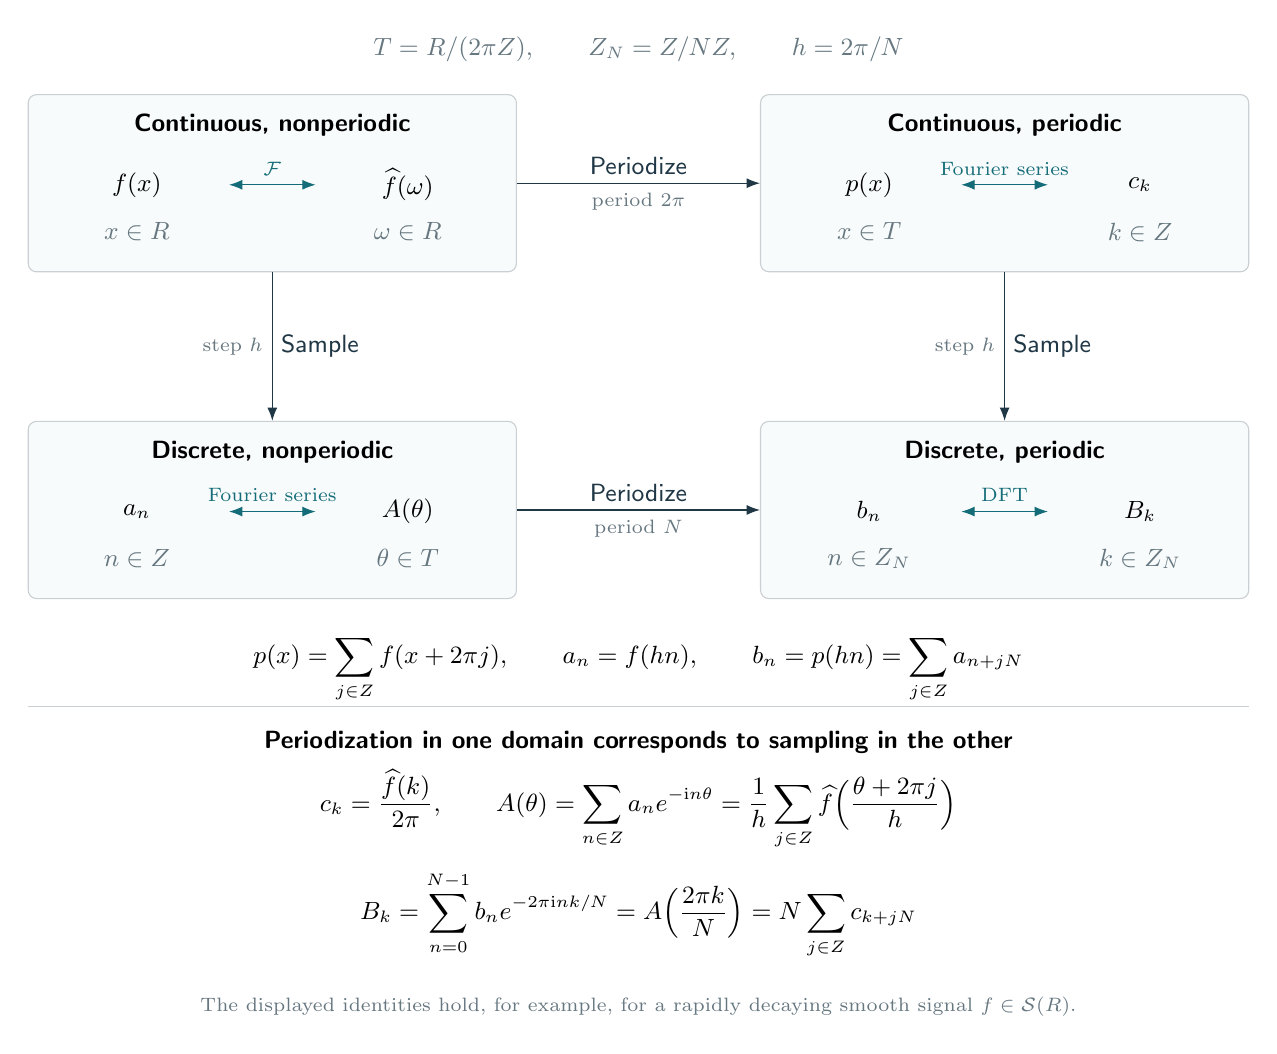
\begin{tikzpicture}[
  setting/.style={draw=muted!35,fill=accent!3,rounded corners=3pt,
    minimum width=6.2cm,minimum height=2.25cm},
  heading/.style={font=\small\sffamily\bfseries},
  operation/.style={font=\small\sffamily,fill=white,inner sep=3pt},
  every node/.style={font=\small}]

\node[setting] (line) at (0,0) {};
\node[setting] (circle) at (9.3,0) {};
\node[setting] (sequence) at (0,-4.15) {};
\node[setting] (finite) at (9.3,-4.15) {};

\foreach \xx/\yy/\title in {
  0/0/{Continuous, nonperiodic},
  9.3/0/{Continuous, periodic},
  0/-4.15/{Discrete, nonperiodic},
  9.3/-4.15/{Discrete, periodic}}{
  \node[heading] at (\xx,\yy+.73) {\title};
}

% Each card pairs a signal with its Fourier representation.
\node at (-1.72,-.02) {$f(x)$};
\node at (1.72,-.02) {$\widehat f(\omega)$};
\node[muted] at (-1.72,-.62) {$x\in\mathbb R$};
\node[muted] at (1.72,-.62) {$\omega\in\mathbb R$};
\draw[<->,accent] (-.55,-.02)--node[above,font=\scriptsize] {$\mathcal F$}(.55,-.02);

\node at (7.58,-.02) {$p(x)$};
\node at (11.02,-.02) {$c_k$};
\node[muted] at (7.58,-.62) {$x\in\mathbb T$};
\node[muted] at (11.02,-.62) {$k\in\mathbb Z$};
\draw[<->,accent] (8.75,-.02)--node[above,font=\scriptsize,align=center] {Fourier series}(9.85,-.02);

\node at (-1.72,-4.17) {$a_n$};
\node at (1.72,-4.17) {$A(\theta)$};
\node[muted] at (-1.72,-4.77) {$n\in\mathbb Z$};
\node[muted] at (1.72,-4.77) {$\theta\in\mathbb T$};
\draw[<->,accent] (-.55,-4.17)--node[above,font=\scriptsize,align=center] {Fourier series}(.55,-4.17);

\node at (7.58,-4.17) {$b_n$};
\node at (11.02,-4.17) {$B_k$};
\node[muted] at (7.58,-4.77) {$n\in\mathbb Z_N$};
\node[muted] at (11.02,-4.77) {$k\in\mathbb Z_N$};
\draw[<->,accent] (8.75,-4.17)--node[above,font=\scriptsize] {DFT}(9.85,-4.17);

% Spatial operations; both routes produce the same finite periodic signal.
\draw[->,ink] (line.east)--node[operation,above] {Periodize}
  node[below,font=\scriptsize,muted] {period $2\pi$}(circle.west);
\draw[->,ink] (sequence.east)--node[operation,above] {Periodize}
  node[below,font=\scriptsize,muted] {period $N$}(finite.west);
\draw[->,ink] (line.south)--node[operation,right] {Sample}
  node[left,font=\scriptsize,muted] {step $h$}(sequence.north);
\draw[->,ink] (circle.south)--node[operation,right] {Sample}
  node[left,font=\scriptsize,muted] {step $h$}(finite.north);

\node[muted] at (4.65,1.7)
  {$\mathbb T=\mathbb R/(2\pi\mathbb Z),\qquad
    \mathbb Z_N=\mathbb Z/N\mathbb Z,\qquad h=2\pi/N$};

\node[anchor=north,align=center,font=\small] at (4.65,-5.62) {
  $\displaystyle p(x)=\sum_{j\in\mathbb Z} f(x+2\pi j),\qquad
    a_n=f(hn),\qquad b_n=p(hn)=\sum_{j\in\mathbb Z}a_{n+jN}$};

\draw[muted!35] (-3.1,-6.65)--(12.4,-6.65);
\node[heading,anchor=north] at (4.65,-6.83)
  {Periodization in one domain corresponds to sampling in the other};
\node[anchor=north,align=center,font=\small] (frequencyrelations) at (4.65,-7.32) {
  $\displaystyle c_k=\frac{\widehat f(k)}{2\pi},\qquad
    A(\theta)=\sum_{n\in\mathbb Z}a_n e^{-\mathrm i n\theta}
      =\frac1h\sum_{j\in\mathbb Z}\widehat f\!\left(\frac{\theta+2\pi j}{h}\right)$\\[7pt]
  $\displaystyle B_k=\sum_{n=0}^{N-1}b_n e^{-2\pi\mathrm i nk/N}
    =A\!\left(\frac{2\pi k}{N}\right)=N\sum_{j\in\mathbb Z}c_{k+jN}$};
\node[muted,font=\scriptsize,below=7pt of frequencyrelations.south]
  {The displayed identities hold, for example, for a rapidly decaying smooth signal $f\in\mathcal S(\mathbb R)$.};
\end{tikzpicture}
\end{document}
